\chapter{Equations and Functions: From Finding One Answer to Studying Them All}

\section{A Taxi Meter and a Cage of Chickens and Rabbits}

Rain starts falling at dusk, and you hail a taxi. As you settle in, a number appears on the meter: 11. The car moves, and you watch the little red screen. At first it ignores you. After a certain distance, it starts clicking upward at intervals, adding 2 yuan each time. At your destination it stops at 21 yuan.

The driver explains the simple rule: the initial fare is 11 yuan for 3 kilometres; beyond that, each kilometre adds 2 yuan. Suddenly you wonder: how far did you just travel?

Even a primary school student could attempt this question. But change it a little: what if the meter shows 35 yuan, or 100 yuan? What if the company changes its rule to 13 yuan for the first 2 kilometres and 3 yuan per kilometre afterward? Every change requires a fresh calculation. Is there a method that handles all such problems at once?

Now consider an old problem that has appeared in Chinese arithmetic books for over a thousand years. A cage contains chickens and rabbits. Count from above and there are 35 heads; count from below and there are 94 legs. How many chickens and rabbits are there? No price or charging rule is given, only two tangled pieces of information. Before reading on, make an intuitive guess: are there more chickens or rabbits? Roughly how many of each?

The meter and the cage seem unrelated: one concerns money, the other animals. By the end of this chapter, you will see them as two faces of the same mathematical family. Learning to recognize that family takes us beyond finding a single answer into a broader landscape: studying the patterns of all answers.

\section{Guessing Until Nightfall: The Failure of Trial and Error}

The natural response to the cage problem is to guess. Suppose all 35 animals are chickens. They have $35 \times 2 = 70$ legs, 24 short of 94, so we need some rabbits. Try 20 chickens and 15 rabbits: $20 \times 2 + 15 \times 4 = 100$ legs, 6 too many. Adjust to 23 chickens and 12 rabbits: $23 \times 2 + 12 \times 4 = 94$. A hit! There are 23 chickens and 12 rabbits.

Getting the answer feels good. But recall the process honestly: each guess took two or three multiplications and an addition, and a wrong guess meant starting again. Would you still want to guess with 3500 heads and 9400 legs? More fundamentally, guessing depends on luck and patience rather than a reliable method. You cannot promise someone that following these steps will certainly find the answer. You can only say that enough attempts will probably hit it.

The taxi problem is similar. Try 5 kilometres: $11 + 2 \times (5-3) = 15$ yuan, too little. Try 10: $11 + 2 \times (10-3) = 25$ yuan, too much. Try 8: $11 + 2 \times (8-3) = 21$ yuan, just right. Three attempts, each like searching for a key in the dark.

Chapter 1 showed the power of letters: a letter can represent any number, allowing one equality to summarize infinitely many specific problems. Our first major step here is to turn guessing into translation. Translate the problem into equalities, then let the equalities tell us the answer.

\section{Translating Problems into Equalities}

Start with the taxi. What we do not know is the distance in kilometres, so name it $x$. Naming an unknown is itself an invention: an invisible quantity becomes a symbol we can manipulate on paper.

The charging rule has two parts. The first 3 kilometres cost a fixed 11 yuan; the extra distance, $(x - 3)$ kilometres, costs 2 yuan per kilometre. Thus ``the fare is 21 yuan'' translates into
\[
11 + 2(x - 3) = 21.
\]
An equality containing an unknown is an \textbf{equation}. Its two sides resemble the pans of a balance. Operations that preserve the balance---adding or subtracting the same number, or multiplying or dividing by the same nonzero number on both sides---preserve the equality. Using that principle,
\[
2(x - 3) = 10,\qquad x - 3 = 5,\qquad x = 8.
\]
The journey was 8 kilometres. This time we deduced it. If the fare were 35 yuan, we would replace 21 by 35 and follow the same steps. If the charging rule changed, we would change the equation's numbers. An equation compresses infinitely many fare questions into one line.

Does the cage problem have just one unknown? It has two: the number of chickens and the number of rabbits. Name them $x$ and $y$. The two given conditions translate into two equations:
\[
\begin{cases}
x + y = 35,\\
2x + 4y = 94.
\end{cases}
\]
Equations bound together form a \textbf{system of equations}. A simple idea solves it: use one equation to replace an unknown. From the first, $y = 35 - x$. Substitute into the second:
\[
2x + 4(35 - x) = 94,\qquad 140 - 2x = 94,\qquad x = 23,
\]
so $y = 35 - 23 = 12$. This matches our guess, but now we know the answer is right and unique, because every reasoning step can be checked.

An elegant old solution imagines a whistle blowing and every animal raising two legs. There are now $94 - 35 \times 2 = 24$ legs on the ground. The chickens are sitting down; only rabbits remain standing, each on two legs. Thus there are $24 \div 2 = 12$ rabbits. Delightful ingenuity---but notice that it does the same work as elimination. Subtract twice $x + y = 35$ from $2x + 4y = 94$, and you remove exactly the two-legs-per-animal contribution. Ingenuity solves one problem; equations solve a class. Ingenuity is the scenery and equations are the road. Mathematics favors roads without rejecting scenery.

In these equations, unknowns appear only to the first power, with no squares or cubes. Hence we call them linear equations in one unknown or systems of linear equations in two unknowns. Are all problems so obliging?

Suppose your family wants to enclose a rectangular vegetable garden with 20 metres of fencing and an area of exactly 24 square metres. What are its dimensions? Let the length be $x$ metres. The width is $(10 - x)$ metres, since length plus width equals half the perimeter. The area condition becomes
\[
x(10 - x) = 24,\qquad \text{which rearranges to}\qquad x^2 - 10x + 24 = 0.
\]
Now the unknown is squared! Simply balancing and isolating terms is not enough: you cannot combine $x^2$ and $x$ as like terms and divide. We are stuck, which is precisely the situation mathematicians find most interesting.

\section{Completing the Square: A Universal Key to Quadratics}

For $x^2 - 10x + 24 = 0$, first try factoring. Can two numbers have product 24 and sum 10? A few attempts find 4 and 6. Thus
\[
x^2 - 10x + 24 = (x - 4)(x - 6) = 0.
\]
A product is zero only if at least one factor is zero, so $x = 4$ or $x = 6$. Length 6 metres and width 4 metres, or vice versa, gives area $6 \times 4 = 24$. The check succeeds.

But this approach has a weakness: we must happen to find the right numbers. What about $x^2 - 10x + 23 = 0$? No two integers have product 23 and sum 10. Does that mean no solution? Not necessarily; perhaps the answers are nonintegers. We need a method independent of guessing.

That method is \textbf{completing the square}. Its central idea comes from a familiar identity, $(x + a)^2 = x^2 + 2ax + a^2$. Read it backward: adding $a^2$ to $x^2 + 2ax$ completes a perfect square. In $x^2 - 10x + 23 = 0$, the initial terms $x^2 - 10x$ give $2a = -10$, so $a = -5$ and the required square is $25$. Add 2 to both sides, turning 23 into 25:
\[
x^2 - 10x + 25 = 2,\qquad (x - 5)^2 = 2,\qquad x - 5 = \pm\sqrt{2}.
\]
Thus $x = 5 + \sqrt{2}$ or $x = 5 - \sqrt{2}$, approximately 6.41 and 3.59. Noninteger answers are within reach too. The value of completing the square is its equal treatment of every quadratic equation. Apply the procedure to the most general quadratic and we obtain this chapter's central theorem.

\begin{dingli}[The Quadratic Formula]
Let $a \neq 0$. When $b^2 - 4ac \geq 0$, all real solutions of $ax^2 + bx + c = 0$ are
\[
x = \frac{-b \pm \sqrt{b^2 - 4ac}}{2a}.
\]
When $b^2 - 4ac = 0$, the two solutions coincide. When $b^2 - 4ac < 0$, there are no real solutions.
\end{dingli}

\begin{proof}
Since $a \neq 0$, divide both sides by $a$:
\[
x^2 + \frac{b}{a}x + \frac{c}{a} = 0.
\]
The coefficient of the linear term is $\dfrac{b}{a}$, so completing the square requires the square of half that coefficient, $\left(\dfrac{b}{2a}\right)^2$. Add the completing term and move $\dfrac{c}{a}$ to the right:
\[
x^2 + \frac{b}{a}x + \left(\frac{b}{2a}\right)^2 = \left(\frac{b}{2a}\right)^2 - \frac{c}{a}
= \frac{b^2}{4a^2} - \frac{4ac}{4a^2} = \frac{b^2 - 4ac}{4a^2}.
\]
The left-hand side is a perfect square:
\[
\left(x + \frac{b}{2a}\right)^2 = \frac{b^2 - 4ac}{4a^2}.
\]
A real square cannot be negative, so the right side must be nonnegative. This gives the condition $b^2 - 4ac \geq 0$. When it holds, take square roots, remembering both signs:
\[
x + \frac{b}{2a} = \pm\frac{\sqrt{b^2 - 4ac}}{2a},
\]
then move $\dfrac{b}{2a}$ to the right and combine over a common denominator to obtain the result.
\end{proof}

This formula deserves respect. Centuries ago, mathematicians argued, wagered, and dueled over equation-solving formulas---actual duels did occur, in the story of cubics that Chapter 5 will tell. Today the formula rests quietly on your page. The expression $b^2 - 4ac$ has its own name, the \textbf{discriminant}. Like a diagnostic reading, its sign tells you whether the equation has real solutions before you calculate them.

\begin{li}
Solve $2x^2 - 7x + 3 = 0$ with the quadratic formula. Here $a = 2$, $b = -7$, $c = 3$, and the discriminant is $49 - 24 = 25 > 0$. Thus
\[
x = \frac{7 \pm 5}{4},\qquad x_1 = 3,\quad x_2 = \frac{1}{2}.
\]
Check in the original equation: $2 \times 9 - 7 \times 3 + 3 = 0$ and $2 \times \frac{1}{4} - 7 \times \frac{1}{2} + 3 = 0$. Both hold.
\end{li}

\section{From Finding One Answer to Studying Them All}

So far, we have repeatedly found the number or numbers satisfying a given condition. That is the equation-solving perspective.

Return to the taxi. A fare of 21 yuan corresponds to 8 kilometres; 35 yuan corresponds to 15 kilometres. We could keep solving forever, gaining only one point each time. Can we present the whole relationship between distance and fare at once?

Yes. For distance $x \geq 3$, the fare is $11 + 2(x - 3)$, or $2x + 5$. This expression is no longer one answer but a \textbf{rule}. Give it any allowed distance and it returns a fare: 4 gives 13, 10 gives 25, 100 gives 205. The rule pairs infinitely many inputs with outputs like a machine that never stops.

Such a rule has a mathematical name, perhaps the most important name in all of secondary-school mathematics.

\begin{shuyu}{Function}
\textbf{Intuitive explanation}: An input-output machine. Put a number in and a number comes out. The same input always gives the same output.

\textbf{Formal definition}: Consider quantities $x$ and $y$. If each value of $x$ in a specified domain corresponds to exactly one determined value of $y$, then $y$ is a function of $x$, written $y = f(x)$. The quantity $x$ is the independent variable, and $f$ denotes the correspondence rule.

\textbf{An example}: $f(x) = 2x + 5$ is the meter's rule for $x \geq 3$: $f(4) = 13$ and $f(10) = 25$.
\end{shuyu}

At first, $f(x)$ can feel awkward. Are $f$ and $x$ being multiplied? No. Read it as ``the value of $f$ at $x$'': the result of putting $x$ through the rule $f$. Previously we could only refer vaguely to a relationship. Now we can name each machine: $f$ might be the meter, $g$ a temperature conversion, and $h$ a phone plan. Then we can compare and combine them.

A function machine has three portraits: a formula such as $f(x) = 2x + 5$, a table of inputs and outputs, and a graph plotting each pair as a point. Formulas are precise, tables concrete, and graphs visual. They are three faces of one rule, and we will move repeatedly between them.

Notice the definition's phrase ``exactly one.'' A machine that sometimes outputs 5 and sometimes 7 for the same input is not a function; it is a faulty machine. Different inputs giving the same output are perfectly acceptable. A machine that tells each person today's day of the week gives everyone the same answer.

Moving from equations to functions is a major shift in viewpoint. An equation asks which $x$ makes $2x + 5 = 21$ true, focusing on one value. A function asks what the rule $f(x) = 2x + 5$ looks like, whether it changes faster or slower, and whether it has a maximum or minimum. Its gaze spans all values. One is a detective search for a particular suspect; the other studies a city's map. In the second half of this chapter, we learn to read maps.

\section{Graphs: The Tracks Left by Rules}

A machine's input and output form a number pair, such as $(4, 13)$ or $(10, 25)$. An ordered pair is exactly a point on coordinate paper. Plot every point produced by a function and you obtain its \textbf{graph}. Think of it as the rule's tracks, like footprints in snow revealing where it goes.

\begin{center}
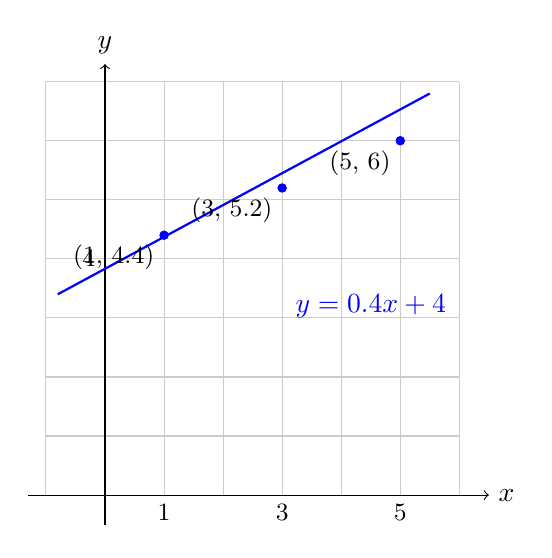
\begin{tikzpicture}[scale=0.75]
\draw[gray!40, step=1] (-1,0) grid (6,7);
\draw[->] (-1.3,0) -- (6.5,0) node[right] {$x$};
\draw[->] (0,-0.5) -- (0,7.3) node[above] {$y$};
\draw[blue, thick] (-0.8,3.4) -- (5.5,6.8);
\filldraw[blue] (1,4.4) circle (2pt) node[below left, black] {\small $(1,\,4.4)$};
\filldraw[blue] (3,5.2) circle (2pt) node[below left, black] {\small $(3,\,5.2)$};
\filldraw[blue] (5,6) circle (2pt) node[below left, black] {\small $(5,\,6)$};
\node[blue] at (4.5,3.2) {$y = 0.4x + 4$};
\node[below] at (1,0) {\small $1$};
\node[below] at (3,0) {\small $3$};
\node[below] at (5,0) {\small $5$};
\node[left] at (0,4) {\small $4$};
\end{tikzpicture}
\end{center}

The figure shows the line $y = 0.4x + 4$. Why is its track straight? Look at the rule: each increase of 1 in $x$ adds 0.4 to $y$; an increase of 5 adds 2. The rate of change is constant, so the track cannot bend. Functions of the form $y = kx + b$, with fixed $k,b$ and $k \neq 0$, are called \textbf{linear functions}; their graphs are straight lines.

Try a different rule: $y = x^2$. Plot a few points:

\begin{center}
\begin{tabular}{cccccccc}
\toprule
$x$ & $-3$ & $-2$ & $-1$ & $0$ & $1$ & $2$ & $3$ \\
\midrule
$y$ & $9$ & $4$ & $1$ & $0$ & $1$ & $4$ & $9$ \\
\bottomrule
\end{tabular}
\end{center}

Notice the symmetry: $(-2, 4)$ and $(2, 4)$ have the same height. Connect the points. To fit the page, we draw the scaled and shifted version $y = \dfrac{1}{2}x^2 - 4$:

\begin{center}
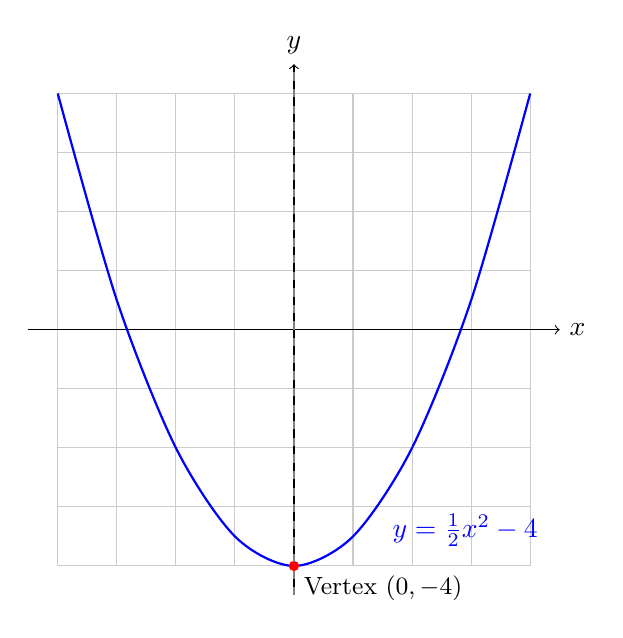
\begin{tikzpicture}[scale=0.75]
\draw[gray!40, step=1] (-4,-4) grid (4,4);
\draw[->] (-4.5,0) -- (4.5,0) node[right] {$x$};
\draw[->] (0,-4.5) -- (0,4.5) node[above] {$y$};
\draw[blue, thick] plot[smooth] coordinates {(-4,4) (-3,0.5) (-2,-2) (-1,-3.5) (0,-4) (1,-3.5) (2,-2) (3,0.5) (4,4)};
\filldraw[red] (0,-4) circle (2.2pt) node[below right, black] {\small Vertex $(0,-4)$};
\draw[dashed, gray] (0,-4.5) -- (0,4.5);
\node[blue] at (2.9,-3.4) {$y = \frac{1}{2}x^2 - 4$};
\end{tikzpicture}
\end{center}

This curve is a \textbf{parabola}. The table explains why it is not straight. From $x=0$ to 1, $y$ moves only a little; from $x=2$ to 3, it jumps much farther. The rate of change increases, so the track bends. A ball thrown into the air and a fountain's jet follow this curve, which is why it looks familiar.

Another relationship worth meeting is \textbf{inverse proportion}. A class pays 300 yuan to hire a vehicle for an outing. The fare per person depends on the number attending, $x$: $y = \dfrac{300}{x}$. With 10 people, each pays 30 yuan; with 30, each pays 10; with 60, each pays 5. More people means a lower price, but the drop slows. Going from 10 to 20 people reduces each fare by 15 yuan; going from 50 to 60 reduces it by only 1 yuan. The graph approaches the axes ever more closely without touching them; it is one branch of a hyperbola. Speed and time for a fixed distance, and length and width for a fixed rectangle area, are also inversely proportional.

Lines, parabolas, and hyperbolas: three tracks, three temperaments. A line changes steadily; a parabola's rate changes; a positive reciprocal curve drops steeply and then flattens. Why draw a graph when we already know the rule? Because our eyes and brains process shapes faster than numbers. We can see whether a curve rises or falls, is steep or gentle, and has high or low points. Extracting the same information from a formula takes work. A graph gives a rule a visual examination.

\section{Slope and Intercept: Reading a Function's Character}

In a line's equation $y = kx + b$, what do $k$ and $b$ control?

Start with $b$. When $x = 0$, $y = b$, so $b$ is the height where the line meets the $y$-axis, called the \textbf{intercept}. In a taxi example, an intercept resembles a fixed charge, the part of the bill present before distance-dependent charges are added.

Now $k$. Each increase of 1 in $x$ increases $y$ by $k$, so $k$ measures the line's \textbf{steepness}. It is the \textbf{slope}. Positive slope means uphill from left to right; negative slope means downhill. Greater absolute slope means a steeper line.

\begin{shuyu}{Slope}
\textbf{Intuitive explanation}: A line's gradient: the vertical rise for each horizontal unit.

\textbf{Formal definition}: For any two points $(x_1, y_1)$ and $(x_2, y_2)$ on a nonvertical line, with $x_1 \neq x_2$, its slope is
\[
k = \frac{y_2 - y_1}{x_2 - x_1}.
\]

\textbf{An example}: Through $(1, 4)$ and $(5, 12)$, the slope is $k = \dfrac{12 - 4}{5 - 1} = 2$: move 1 right and rise 2.
\end{shuyu}

An important fact hides in the definition: the ratio is \textbf{independent} of the two points chosen. Why should different points give the same slope? Because a linear function changes at a constant rate: $y_2 - y_1 = kx_2 + b - (kx_1 + b) = k(x_2 - x_1)$. Division gives exactly $k$, with $b$ canceled. Conversely, if a function's slope varies with position, its graph cannot be a line. That is why a parabola is gentle near its bottom and steeper farther up.

Slope has another important name: \textbf{rate of change}. A distance-fare line of slope 2 means 2 yuan per kilometre. The slope of a time-distance line is speed; the slope of a time-savings line is the saving rate. Understanding slope means understanding how quickly something changes.

Slope also carries units, an easily overlooked but useful fact. Fare against distance has units of yuan per kilometre; distance against time has units of metres per second. The units themselves explain what the rate measures. Negative slopes matter too. Altitude against time has positive slope while climbing and negative slope while descending; body temperature rises with a developing fever and falls as the fever subsides. The sign tells us whether the quantity increases or decreases.

\begin{fanli}
``$y$ increases as $x$ increases, so they are directly proportional.'' False. Consider $y = x + 1$. As $x$ goes from 1 to 2, $y$ goes from 2 to 3, so it increases. But the ratio of $y$ to $x$ changes from 2 to 1.5, and at $x = 0$, $y$ is not 0. Direct proportion requires a line through the origin, with $b = 0$. A related trap is ``the graph rises, so it is a straight line.'' The parabola $y = x^2$ also rises throughout $x > 0$, yet it curves. Rising describes direction, not shape.
\end{fanli}

The inverse-proportion function $y = \dfrac{300}{x}$ has a different character. It has no single uniform slope: near the origin it is extremely steep, while farther away it is almost flat. The rate of change itself changes. Acknowledging this was a deep breath in mathematical history, and Chapter 10 will face it directly.

\section{A Different Perspective: Let Graphs Speak for Equations}

Once we can read graphs, equations look different.

The equation $2x + 5 = 21$ asks for the horizontal coordinate where $y = 2x + 5$ reaches height 21. The system
\[
\begin{cases}
y = 2x + 5,\\
y = -x + 23
\end{cases}
\]
asks where two lines intersect. Draw them: two nonparallel lines meet at exactly one point. That is the geometric reason a two-variable linear system typically has a unique solution. The equation $x^2 - 10x + 24 = 0$ asks where the parabola $y = x^2 - 10x + 24$ meets the ground, or $x$-axis. A positive discriminant gives two crossings; zero gives one touch before the curve rises again; a negative discriminant leaves this upward-opening parabola suspended above the ground. No real solution means no contact.

\begin{lianjie}
In Chapter 1, letters compressed arithmetic problems into algebraic expressions. Here graphs translate expressions back into shapes. Equations, functions, and graphs are three languages for the same underlying relationship. An equation interrogates it for particular values of $x$; a function describes the whole correspondence; a graph maps that correspondence. Chapter 4 will connect this translation system fully by turning geometric shapes directly into algebraic equations. But why trust the points, lines, and angles in a picture? Why does an apparent intersection count as a real one? Chapter 3 will answer through proof.
\end{lianjie}

Changing languages has practical power. A list of monthly electricity bills for the past year may reveal little at first glance. Plot them and trends, anomalies, and cycles emerge. Temperature curves in weather forecasts, fluctuations in stock displays, and growth curves in health reports all illustrate the same idea: rules leave tracks, and tracks reveal rules.

The reverse works too: translate a geometric problem into equations. A park fountain sends water along a parabola. The designer wants it to return to the pool 4 metres away and reach a maximum height of 2 metres. These shape requirements become equations whose solutions determine precise nozzle parameters. Shapes set requirements and equations supply answers, as engineers do every day. Chapter 4 practises this translation systematically.

\begin{shiyan}
\textbf{Experiment one: draw your own parabola.} Plot 9 points of $y = x^2$ for $x$ from $-4$ to $4$ on squared paper and connect them with a smooth curve. Then (1) fold along the $y$-axis to check whether the halves coincide, and (2) use a ruler to compare the curve's slope near $(1,1)$ and $(3,9)$, feeling how slope changes with position.

\textbf{Experiment two: measure an everyday slope.} Find some stairs and measure one step's height and depth, perhaps 15 and 28 centimetres. Calculate the gradient: $15 \div 28 \approx 0.54$. Make the same measurements on an accessible ramp and compare. You have done the same work as an engineer designing a ramp or a mathematician defining slope.
\end{shiyan}

\begin{toolbox}
Your new tools from this chapter:
\begin{itemize}
\item \textbf{Setting up equations}: Name unknowns and translate conditions into equalities. For several unknowns, use a system and eliminate by substitution.
\item \textbf{Completing the square and the quadratic formula}: A general procedure for quadratic equations. The discriminant $b^2 - 4ac$ first reports whether real solutions exist.
\item \textbf{Function notation $f(x)$}: Treat a correspondence rule as an object you can name and study.
\item \textbf{Graphs}: Plot points to turn rules into visible tracks. Lines, parabolas, and hyperbolas are three common examples.
\item \textbf{Slope and intercept}: Two parameters of a linear function, controlling steepness and starting position. Slope is rate of change.
\end{itemize}
\end{toolbox}

\begin{pandeng}
Farther along, these ideas await: \textbf{growth rates and derivatives}, with Chapter 10 defining instantaneous slope at each point of a parabola; \textbf{composition and inverse functions}, connecting machines in series or running one backward; \textbf{exponential and logarithmic functions}, including relationships whose growth rate itself grows, such as bacteria populations and savings; and \textbf{fixed points}, inputs a machine returns unchanged. University mathematics extends functions to astonishing settings. We can speak of distances between functions, and collections of functions can themselves form spaces.
\end{pandeng}

\section*{Reflection Questions}

\textbf{Observation}
\begin{sikao}
\item Draw $y = 2x + 5$ and $y = -x + 23$ on the same axes, locate their intersection, and solve the system. How do the intersection coordinates relate to the solution, and why? \emph{Hint: the intersection lies on both lines, so its coordinates satisfy both rules.}
\item For $y = \dfrac{12}{x}$, how much does $y$ change as $x$ goes from 1 to 2? What about from 6 to 7? Why are the changes so different for equal input intervals? \emph{Hint: calculate the actual $y$ values and compare the changes, rather than starting with rates.}
\end{sikao}

\textbf{Proof}
\begin{sikao}
\item Prove that two positive numbers with sum 10 have product at most 25, with equality only when both are 5. \emph{Hint: write them as $x$ and $10 - x$, express their product as a quadratic, and complete the square. Recall the garden problem.}
\item Let $f(x) = kx + b$ with $k > 0$. Prove that $x_1 < x_2$ implies $f(x_1) < f(x_2)$, a property called strict monotonic increase. \emph{Hint: calculate $f(x_2) - f(x_1)$ and use $x_2 - x_1 > 0$ and $k > 0$ to determine its sign.}
\end{sikao}

\textbf{Challenge}
\begin{sikao}
\item Let $x_1,x_2$ be the two solutions of $ax^2 + bx + c = 0$. Without evaluating them individually, prove $x_1 + x_2 = -\dfrac{b}{a}$ and $x_1 x_2 = \dfrac{c}{a}$. \emph{Hint: add and multiply the two expressions in the quadratic formula, watching how $\sqrt{\phantom{a}}$ disappears. Chapter 5 gives these relationships a name.}
\item A city's taxi rule charges 11 yuan within 3 kilometres, 2 yuan per kilometre from 3 to 10 kilometres, and 3 yuan per kilometre beyond 10. Write the fare $y$ as a piecewise expression in distance $x$ and draw its graph. Is this machine a function? What happens at $x = 3$ and $x = 10$? \emph{Hint: check that each input has one output. The graph has no break, but its slope changes suddenly; such points will later have a special name.}
\end{sikao}

\section*{The Door to the Next Chapter}

This chapter has built a habit: turn relationships into graphs and view equations through intersections. Graphs have become our trusted eyes.

But recall one small detail. To draw the parabola, you plotted 9 points and connected them with a smooth curve. Why was that justified? You saw nine points roughly following a curved track and joined them. Perhaps the curve secretly bends between two points in a way you missed. Perhaps lines that seem to intersect at $(6, 17)$ measure as $(5.98, 17.03)$. Eyes and rulers reveal clues, but never guarantee a conclusion. That is the boundary between measurement and proof.

Next we return to mathematics older than functions: points, lines, angles, triangles, and circles. We will see how the ancient Greeks began with the impossibility of drawing a perfect straight line and built humanity's first great structure of proof. We will also ask why the same conclusion, such as the famous theorem about a right triangle's sides, deserves a dozen different proofs. Graphs let us see an answer; proofs let us be sure. Now let us meet the second.
